In questa esperienza si vuole realizzare un misuratore di distanza utilizzando il sensore di distanza a ultrasuoni HC-SR04, il cui pinout è riportato in Figura \ref{fig:HC-SR04}. Si vuole utilizzare il sensore in modo "nativo", senza utilizzare librerie già scritte. Sono stati utilizzati i seguenti componenti:
\begin{itemize}
    \item Scheda Arduino DUE, breadboard e cavi.
    \item Display TFT 3.5" 320x480, \textit{HX8357} Adafruit
    \item Sensore ultrasonico distanza HC-SR04
\end{itemize}
Il circuito è alimentato mediante porta USB del PC, la quale eroga circa $(\sim 5 V)$. Il sensore HC-SR04 è alimentato con una tensione di $V_{CC}=5$ V. Per garantire la sicurezza degli ingressi della scheda Arduino Due, che operano a una tensione di 3.3 V, si è realizzato un semplice partitore di tensione collegato all'uscita del sensore (ECHO). Il partitore di tensione riduce la tensione di uscita del sensore a un valore prossimo a 3.3 V, consentendo così all'Arduino Due di rilevare correttamente il segnale.
\begin{figure}[H]
    \centering
    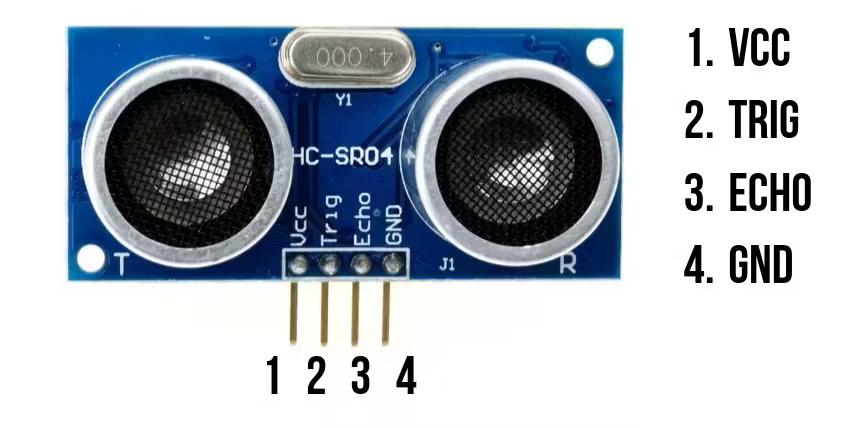
\includegraphics[width=0.5\linewidth]{images/HC-SR04.png}
    \caption{Pinout del sensore HC-SR04}
    \label{fig:HC-SR04}
\end{figure}
\subsection{Codice - Interfaccia grafica}
\begin{lstlisting}[frame=single, language=Arduino]
#include <SPI.h>
#include "Adafruit_GFX.h"
#include "Adafruit_HX8357.h"

#define TRIG_PIN 7
#define ECHO_PIN 6

#define TFT_CS 10
#define TFT_DC 9
Adafruit_HX8357 tft = Adafruit_HX8357(TFT_CS, TFT_DC, -1); 

void setup(){
    pinMode(ECHO_PIN, INPUT);
    pinMode(TRIG_PIN, OUTPUT);
\end{lstlisting}
\begin{lstlisting}[frame=single, language=Arduino]
    // Configurazione del display
    tft.begin();
    tft.setRotation(3);
    tft.fillScreen(HX8357_BLACK);
    tft.setTextColor(HX8357_GREEN);
    tft.setTextSize(6);
    tft.setCursor(60,0);
    tft.println("Distanza");
    tft.setTextColor(HX8357_WHITE);
    tft.setTextSize(10);
}

void loop(){
    String DistTxt = String(distance());
    
    tft.fillRect(0,120,480,320,HX8357_BLACK);
    tft.setCursor(0,150);
    tft.println(DistTxt + " cm");
    
    delay(100);
}
\end{lstlisting}
\subsection{Codice - Lettura sensore HC-SR04}
\begin{lstlisting}[frame=single, language=Arduino]
long distance(){
    long d = 0;
    long duration = 0;
    // Invio dell' inpulso di TRIG
    digitalWrite(TRIG_PIN, LOW);
    delayMicroseconds(2);
    digitalWrite(TRIG_PIN, HIGH);
    delayMicroseconds(2);
    digitalWrite(TRIG_PIN, LOW);
    delayMicroseconds(2);
    // Lettura della durata dell' inpulso da ECHO
    duration = pulseIn(ECHO_PIN, HIGH);
    d = (duration * 100) / 5830;
    delay(25);
    return d;
}
\end{lstlisting}
\clearpage
\noindent La funzione integrata \texttt{pulseIn(pin,value)} ritorna il tempo in microsecondi in cui un determinato \texttt{pin} mantiene il livello \texttt{value}, legge quindi la durata di un inpulso su un pin e ne ritorna la lunghezza in microsecondi. In questo caso fa partire un timer quando il pin \texttt{ECHO\_PIN} commuta a livello \texttt{HIGH} e interrompe il timer quando il pin ritorna a livello \texttt{LOW}, ritornando poi il valore del timer in microsecondi
\begin{figure}[H]
    \centering
    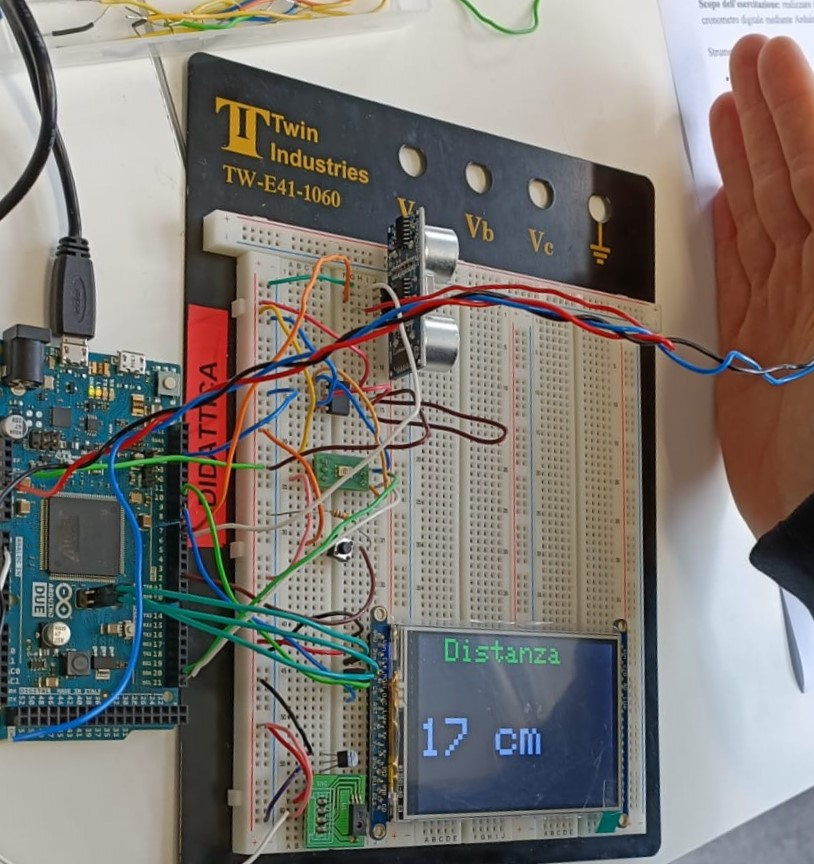
\includegraphics[width=.65\linewidth]{images/IMG-20230519-WA0010.jpg}
    \caption{Prova del funzionamento del sensore}
\end{figure}